\documentclass[a0paper,portrait]{tikzposter}

\usepackage{booktabs}
\usepackage{mathtools}
\usepackage{tikz-cd}
\usepackage{authblk}
\usepackage[export]{adjustbox}

%\addbibresource{../UAI_paper/paper.bib}

\tikzposterlatexaffectionproofoff
\usetheme{Rays}

% TODO: use lots of bold

\makeatletter
\def\title#1{\gdef\@title{\scalebox{\TP@titletextscale}{%
      \begin{minipage}[t]{\linewidth}
        \centering
        #1
        \par
        \vspace{0.5em}
      \end{minipage}%
    }}}
\makeatother

\makeatletter
\newcounter{tablecounter}
\newenvironment{tikztable}[1][]{
  \def \rememberparameter{#1}
  \vspace{10pt}
  \refstepcounter{tablecounter}
  \begin{center}
  }{
    \ifx\rememberparameter\@empty
    \else
    \\[10pt]
    {\small Tab.~\thetablecounter: \rememberparameter}
    \fi
  \end{center}
}
\makeatother

\makeatletter
\def\maketitle{\AB@maketitle}
\makeatother

\title{Weighted Model Counting with Conditional Weights for Bayesian Networks}
\author[1]{Paulius Dilkas}
\author[1,2]{Vaishak Belle}
\affil[1]{School of Informatics, University of Edinburgh, Edinburgh, UK}
\affil[2]{The Alan Turing Institute, London, UK}
\titlegraphic{
\includegraphics[height=200pt,valign=c]{logo_inf.png}\hspace{3em}
\includegraphics[height=200pt,valign=c]{logo_ecr.png}\hspace{3em}
\includegraphics[height=100pt,valign=c]{logo_ukri.png}}

\begin{document}
\maketitle

\begin{columns}
  \column{0.5}
  \block{Boolean Algebras and Propositional Logic}{
    Let $U = \{ a, b \}$. Then $2^{2^U}$ is a Boolean algebra with the following
    Hasse diagram ($x \le y$ if $x \subseteq y$ or, equivalently, $x = x \land
    y$).
    % \[
    %   \begin{tikzcd}[ampersand replacement=\&, column sep=tiny]
    %     \& \& \& \& \& \top \ar[dlll,dash,gray] \ar[dl,dash,gray]
    %     \ar[dr,dash,gray] \ar[drrr,dash,gray] \& \& \& \\
    %     \& \& a \lor b \& \& b \to a \& \& a \to b \& \& \neg a \lor \neg
    %     b \\
    %     a \ar[urr,dash,gray] \ar[urrrr,dash,gray] \& \& b \ar[u,dash,gray]
    %     \ar[urrrr,dash,gray] \& \& a \leftrightarrow b \ar[u,dash,gray]
    %     \ar[urr,dash,gray] \& \& a + b \ar[ullll,dash,gray] \ar[urr,dash,gray]
    %     \& \& \neg b \ar[ullll,dash,gray] \ar[u,dash,gray] \& \& \neg a
    %     \ar[ullll,dash,gray] \ar[ull,dash,gray] \\
    %     \& \& \fbox{$a \land b$} \ar[ull,dash,gray] \ar[u,dash,gray]
    %     \ar[urr,dash,gray] \& \& \fbox{$a \land \neg b$} \ar[ullll,dash,gray]
    %     \ar[urr,dash,gray] \ar[urrrr,dash,gray] \& \& \fbox{$\neg a \land b$}
    %     \ar[ullll,dash,gray] \ar[u,dash,gray] \ar[urrrr,dash,gray] \& \&
    %     \fbox{$\neg a \land \neg b$} \ar[ullll,dash,gray] \ar[u,dash,gray]
    %     \ar[urr,dash,gray] \\
    %     \& \& \& \& \& \bot \ar[ulll,dash,gray] \ar[ul,dash,gray]
    %     \ar[ur,dash,gray] \ar[urrr,dash,gray] \& \& \&
    %   \end{tikzcd}
    % \]
  }

  \block{Experimental Results}{
    \begin{tikzfigure}[Cumulative numbers of instances solved by combinations of
      algorithms and encodings over time.]
      \centering
      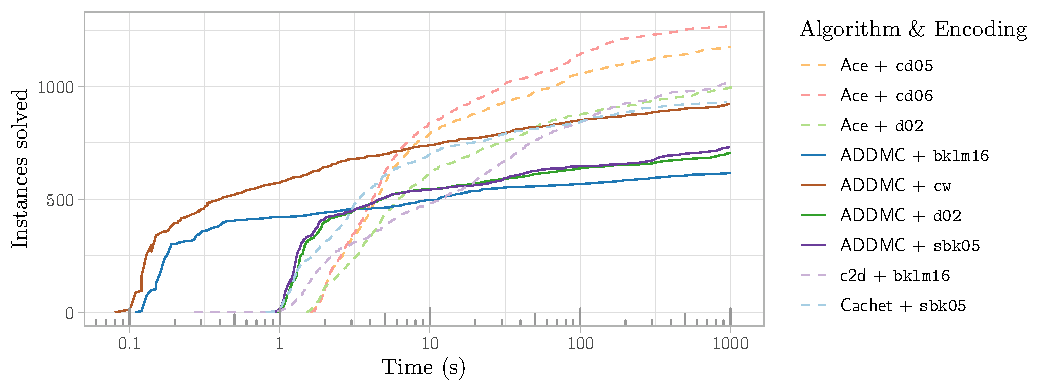
\includegraphics[width=\linewidth]{cumulative}
    \end{tikzfigure}
    \begin{tikzfigure}[An instance-by-instance comparison between
      $\textsf{ADDMC} + \texttt{cw}$ and the best overall combination of
      algorithm and encoding ($\textsf{Ace} + \texttt{cd06}$, on the left) as
      well as the second-best encoding for \textsf{ADDMC} (\texttt{sbk05}, on
      the right).]
      \centering
      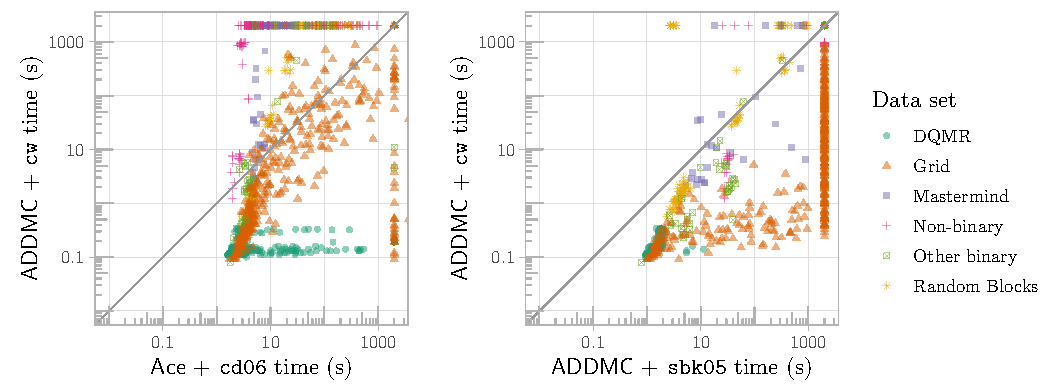
\includegraphics[width=\linewidth]{scatter}
    \end{tikzfigure}
  }

  \column{0.5}

  \block{TODO}{
    \begin{tikztable}[Asymptotic upper bounds on the numbers of variables and
      clauses/ADDs for each encoding.]
      \centering
      \begin{tabular}{l c c}
        \toprule
        Encoding(s) & Variables & Clauses/ADDs \\
        \midrule
        \texttt{bklm16}, \texttt{cd05}, \texttt{cd06}, \texttt{sbk05} & $O(nv^{d+1})$ & $O(nv^{d+1})$ \\
        \texttt{cw} & $O(nv)$ & $O(nv^2)$ \\
        \texttt{d02} & $O(nv^{d+1})$ & $O(ndv^{d+1})$ \\
        \bottomrule
      \end{tabular}
    \end{tikztable}
  }

\end{columns}
\end{document}